\documentclass{article}
\usepackage[brazilian]{babel}
\usepackage[utf8]{inputenc}
\usepackage[T1]{fontenc}
\usepackage[a4paper]{geometry}
\usepackage{amsmath}
\usepackage{amssymb}
\usepackage{indentfirst}
\usepackage{graphicx}
\usepackage{natbib}
\renewcommand{\rmdefault}{ptm}

\title{Relatório EP1}
\author{Beatriz F. Marouelli, Leonardo Lana Violin Oliveira}
\date{23 de Abril de 2017}
\begin{document}

\maketitle

\section*{Parte 1}
\subsection*{Resumo do Programa}

O programa \textit{binary\_arithmetic} usa vetores de 32 posições para
representar os números na notação de ponto flutuante no intervalo normalizado.
O programa possui 9 funções:

\begin{itemize}
    \item \textbf{\textit{btsToDec}}
        \\ Extrai a \textit{bitstring} do vetor e retorna o valor em decimal da mesma.
    
    \item \textbf{\textit{checkNaN}} 
        \\ Checa se um vetor representa um \textit{NaN}.
    
    \item \textbf{\textit{expDiff}}
        \\ Dados dois números, retorna a diferença entre as bitstrings deles.
        Essa diferença é usada para criar um \textit{offset} necessário durante
        as operações e para deteminar qual dos números é o maior e o menor.
    
    \item \textbf{\textit{negateNum}}
        \\ Nega o significando do vetor de acordo com a regra de complemento de
        dois, aplicando um \textit{offset}, se necessário.
    
    \item \textbf{\textit{precisionBits}}
        \\ Transforma o vetor para atender as especificações, ou seja, com dois
        \textit{guard bits} e um \textit{sticky bit}.
    
    \item \textbf{\textit{printVec}}
        \\ Imprime o vetor fornecido no formato \textit{\textbf{<index>} :
            \textbf{<content>}}.
    
    \item \textbf{\textit{signalSetter}}
        \\ Retorna o sinal correto do resultado da operação.
    
    \item \textbf{\textit{round}}
        \\ Retorna 4 vetores, cada um com um arredondamento diferente,
        \textbf{para 0}, \textbf{para o mais próximo}, \textbf{para o $+
        \infty$} e \textbf{para o $- \infty$}.

    \item \textbf{\textit{reSub}}
        \\ Usa a função \textit{\textbf{signalSetter}} para determinar o sinal
        do resultado. Nega o significando do segundo número, usando a 
        \textbf{\textit{negateNum}}. Copia o significando do vetor menor, usando 
        o \textit{offset} dado pela \textit{\textbf{expDiff}}, caso o menor seja 
        o segundo número, copia do vetor fornecido pela \textit{\textbf{negateNum}}.

        Após a cópia, soma os dois significandos \textit{bit} a \textit{bit}.
        
        Após a soma, avalia a flag \textit{carryout} para normalizar o vetor. Caso, a flag 
        seja $2$, será necessário buscar o primeiro \textit{bit} não nulo no
        significando, deslocar o vetor para que este \textit{bit} torne-se o
        oculto, após isto, será necessário subtrair o número de casas deslocadas
        da \textit{bitstring} do maior número, e copiar o resultado para
        \textit{bitstring} do resultado. Caso seja $1$, é necessário apenas subtrair $1$
        no expoente e copiar o resultado dessa subtração para a \textit{bitstring} 
        do resultado. Caso não seja nem $1$ ou $2$, só é necessário copiar a 
        \textit{bitstring} do maior número.
    
    \item \textbf{\textit{reSum}}
        \\ Usa a função \textit{\textbf{signalSetter}} para determinar o sinal
        do resultado. Copia o significando do vetor menor, usando o \textit{offset} 
        dado pela \textit{\textbf{expDiff}}.

        Após a cópia, soma os dois significandos \textit{bit} a \textit{bit}.

        Após a soma, avalia a flag \textit{carryout} para normalizar o vetor.
        Caso, a flag seja maior que $1$, soma-se $1$ à \textit{bitstring} do
        número maior, e desloca o vetor um \textit{bit} para trás. Caso seja 
        igual a $2$, o primeiro bit do significando passa a ser $0$, caso seja 
        igual a $3$, o primeiro bit do significando torna-se $1$.

\end{itemize}

\subsection*{Exemplos}
\begin{itemize}
\item $2 \oplus 3$
    \begin{itemize}
        
    \item \textit{estado inicial} \\    
    $2 = {0}\ {10000000}\ {00000000000000000000000}$ \\
    $3 = {0}\ {10000000}\ {10000000000000000000000}$ \\
    \textit{ret} $= {0}\ {00000000}\ {00000000000000000000000}$ \\

    \item \textit{offset} \\
    ${10000000}\ - {10000000} = 0$
    
    \item \textit{define o sinal} \\
    $ 3 > 2$, logo \textit{ret} $= {0}\ {00000000}\ {00000000000000000000000}$
      
    \item \textit{cópia com offset} \\
    \textit{ret} $= {0}\ {00000000}\ {00000000000000000000000}$
      
    \item \textit{soma com o maior} \\
    \textit{ret} $= {0}\ {00000000}\ {10000000000000000000000}$

    \item \textit{normalização} \\
    \textit{ret} $= {0}\ {00000001}\ {01000000000000000000000}$
    
    \item \textit{cópia do expoente com alterações} \\
    \textit{ret} $= {0}\ {10000001}\ {01000000000000000000000}$

    \item \textit{Como o resultado cabe em formato de floating, todos os rounds serão:} \\
    \textit{ret} $= {0}\ {10000001}\ {01000000000000000000000}$
    \end{itemize}

\item $1 \oplus 2^{-24} $ 
    \begin{itemize}
        
    \item \textit{estado inicial} \\    
    $1 = {0}\ {01111111}\ {00000000000000000000000}$ \\
    $2^{-24} = {0}\ {01100111}\ {10000000000000000000000}$ \\
    \textit{ret} $= {0}\ {00000000}\ {0000000000000000000000000000000000000000000000}$ \\

    \item \textit{offset} \\
    ${01111111}\ - {01100111} = 24$
    
    \item \textit{define o sinal} \\
    $1 > 2^{-24}$, logo \\\
    textit{ret} $= {0}\ {00000000}\ {0000000000000000000000000000000000000000000000}$ 
     
    \item \textit{cópia com offset} \\
    \textit{ret} $= {0}\ {00000000}\ {0000000000000000000000010000000000000000000000}$
      
    \item \textit{soma com o maior} \\
    \textit{ret} $= {0}\ {00000000}\ {0000000000000000000000010000000000000000000000}$
    \textit{carryout} $= 1$

    \item \textit{normalização} \\
    \textit{ret} $= {0}\ {00000000}\ {0000000000000000000000010000000000000000000000}$
    
    \item \textit{cópia do expoente com alterações} \\
    \textit{ret} $= {0}\ {01111111}\ {0000000000000000000000010000000000000000000000}$

    \item \textit{Round Up} \\
    \textit{ret} $= {0}\ {01111111}\ {00000000000000000000001}$

    \item \textit{Round Down, Round towards Zero, Round to the Nearest} \\
    \textit{ret} $= {0}\ {01111111}\ {00000000000000000000000}$
    \end{itemize}

\item $1 \ominus {(1.11111111111111111111111)}_{2} \times 2^{-1}$
    \begin{itemize}
        
    \item \textit{estado inicial} \\    
    $1 = {0}\ {01111111}\ {00000000000000000000000}$ \\
    ${(1.11111111111111111111111)}_{2} \times 2^{-1} = {0}\ {01111110}\ {11111111111111111111111}$ \\
    \textit{ret} $= {0}\ {00000000}\ {000000000000000000000000}$

    \item \textit{offset} \\
    ${01111111}\ - {01111110} = 24$
    
    \item \textit{define o sinal} \\
    $1 > {(1.11111111111111111111111)}_{2} \times 2^{-1}$, logo \\ 
    \textit{ret} $= {0}\ {00000000}\ {000000000000000000000000}$ \\
      
    \item \textit{cópia com offset} \\
    \textit{ret} $= {0}\ {00000000}\ {000000000000000000000001}$ \\
      
    \item \textit{soma com o maior} \\
    \textit{ret} $= {0}\ {00000000}\ {000000000000000000000001}$ \\

    \item \textit{normalização} \\
    \textit{ret} $= {0}\ {0000000-1}\ {000000000000000000000001}$ \\
    
    \item \textit{cópia do expoente com alterações} \\
    \textit{ret} $= {0}\ {01111110}\ {000000000000000000000001}$ \\
    
    \item \textit{Round Up} \\
    \textit{ret} $= {0}\ {01111110}\ {00000000000000000000001}$

    \item \textit{Round Down, Round towards Zero, Round to the Nearest} \\
    \textit{ret} $= {0}\ {01111110}\ {00000000000000000000000}$
    \end{itemize}

\item $1 \ominus {(1.00000000000000000000001)}_{2} \times 2^{-25}$
    \begin{itemize}
        
    \item \textit{estado inicial} \\    
    $1 = {0}\ {01111111}\ {00000000000000000000000}$ \\
    ${(1.00000000000000000000001)}_{2} \times 2^{-25} = {0}\ {01100110}\ {10000000000000000000001}$ \\
    \textit{ret} $= {0}\ {00000000}\ {00000000000000000000000000000000000000000000000}$ \\

    \item \textit{offset} $ {01111111} - {01100110} = 25$
    
    \item \textit{define o sinal} \\
    $1\ > {(1.00000000000000000000001)}_{2} \times 2^{-25}$, logo \\
    \textit{ret} $= {0}\ {00000000}\ {00000000000000000000000000000000000000000000000}$ \\
      
    \item \textit{cópia com offset} \\
    \textit{ret} $= {0}\ {00000000}\ {11111111111111101001100011111111111111111111111}$ \\
      
    \item \textit{soma com o maior} \\
    \textit{ret} $= {0}\ {00000000}\ {11111111111111101001100011111111111111111111111}$ \\

    \item \textit{normalização} \\
    \textit{ret} $= {0}\ {0000000-1}\ {11111111111111101001100011111111111111111111111}$ \\
    
    \item \textit{cópia do expoente com alterações} \\
    \textit{ret} $= {0}\ {01111110}\ {11111111111111101001100011111111111111111111111}$ \\
    
    \item \textit{Round Up} \\
    \textit{ret} $= {0}\ {01111110}\ {11111111111111110100111}$

    \item \textit{Round Down, Round towards Zero, Round to the Nearest} \\
    \textit{ret} $= {0}\ {01111110}\ {11111111111111110100110}$
    \end{itemize}
\end{itemize}

\begin{flushleft}

\end{flushleft}

\section*{Parte 2}
O método de newton consiste num método iterativo para encontrar raízes de uma função, ou seja,
os pontos em que ela é zero. Para aproximar o valor da raiz, o método itera da seguinte maneira: \\
$x_{n+1} = x_{n} - f(x_{n})/f'(x_{n})$, onde $f(x)$ é a função que desejamos aproximar as
raízes e $f'(x)$ sua derivada.

No programa implementado, na função \textit{newton ()}, o método itera até o erro (definido abaixo) 
tenha módulo menor do que $1 \times 10^{-6}$ ou o limite de 10 iterações seja alcançado. Caso esse limite seja alcançado,
o ponto em questão para o qual o método foi testado é marcado como não-convergente.

Muitos testes foram feitos para definir quais seriam os critérios de parada mais adequados para o método,
na sessão de imagem, serão mostrados alguns exemplos de imagens com critérios de parada diferentes do definido na versão final. 

A função \textit{newton\_basins ()} gera um arquivo em formato \textit{.txt}, onde cada linha contém as coordenadas 
do ponto testado pelo método e a raiz para qual ele convergiu, ou a marcação definida, caso ele não tenha
convergido.


E por fim, seguem algumas imagens geradas pelo script (disponibilizado pelo
monitor desta matéria no oferecimento do ano passado) com os resultados obtidos
pela \textit{newton\_basins ()}.


\begin{figure}[h]
\caption{Exemplo de fractal da função $x^{3} - 1$}
\centering
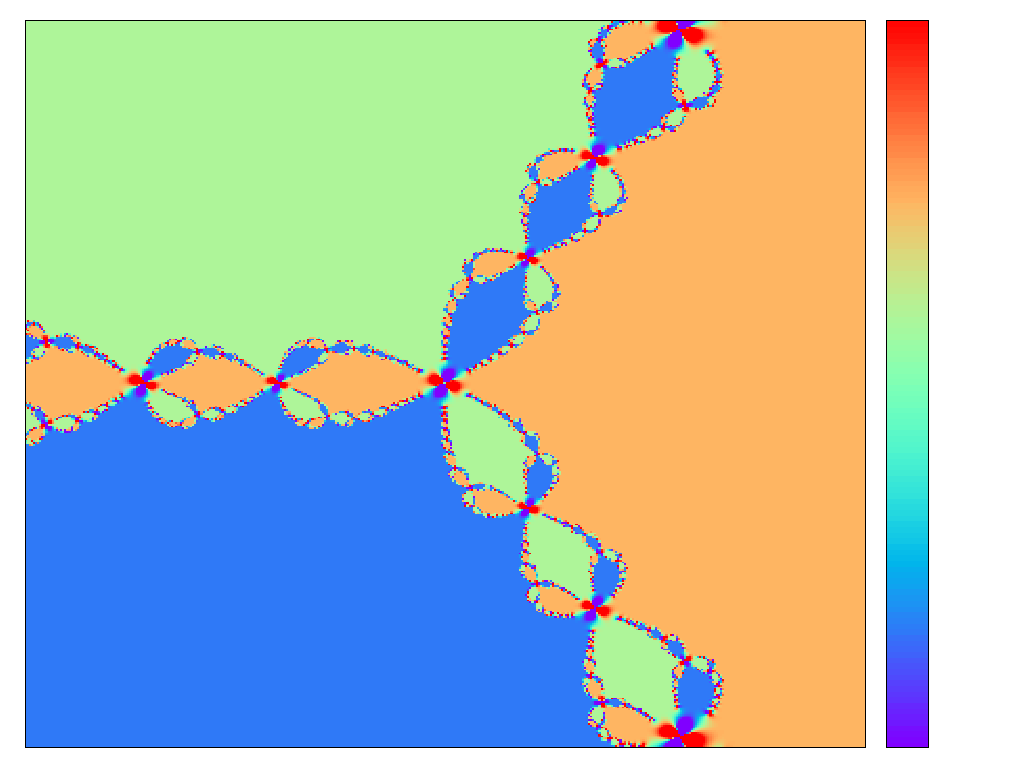
\includegraphics[width=13cm, height=13cm]{newton_basins.png}
\end{figure}


%Figura 2: Exemplo de fractal da função x^5 - 1 (legenda de cima)

%Pode-se notar os pontos marcados em vermelho na imagem, que são os pontos que não convergem.(comentário depois das figuras 1 e 2)

%Figura 3: Fractal da função de x^5 - 1 com número de iterações igual a 10. (legenda de cima)

%Também é fácil notar que a quantidade de pontos que não convergem aumenta devido à mudança do
%critério de parada. (comentário depois)

\end{document}
